\documentclass{jreport}		% 標準のクラスファイル
\usepackage{paper}			% 神戸高専卒論用のマクロ
\usepackage[dvipdfmx]{graphicx}		% eps等図を取り込むためのマクロ
\usepackage[subrefformat=parens]{subcaption}
%\usepackage{times}

\title{LSTMを用いた楽器エフェクタの\\シミュレータ構築}	% 卒業論文のタイトル
\author{氏本 大智}		% 報告者
\adviser{長谷 芳樹}			% 指導教官
\year{30}					% 年度

\abstract{
 現在,音響機器がディジタルでシミュレートされ,ソフトウェアとして実現される場面が多くなっている.音響特性のシミュレート技術も進歩し,数々のシミュレータが開発され,それらは高い再現度を実現している.中でも,ニューラルネットワークを利用したシミュレータの精度の高さが注目されている.
ニューラルネットワークを用いたシミュレートシステムは一般に普及しつつあるが,シミュレートには専用のハードが必要になるケースが多く,ソフトウェア単体で動作するシステムは未だ実用化されていない.\\
 本研究では,PC のみで動作し,エフェクタへの入出力音を入れるだけで音響フィルタを手軽にシミュレートできる,ニューラルネットワークを用いた音響フィルタのシミュレータ開発の検討を行った.\\
 ギターの原音データとひずみエフェクタを通した音声データを用意し,ニューラルネットワークを用いたシミュレータを作成した.その後,作成したシミュレータから得られた出力と教師データ出力の波形の比較,フーリエ変換処理を加え,得られた周波数スペクトルの比較を行った.その結果,出力波形は似かよったものが得られたが,周波数スペクトルをみると,6000Hzから精度が落ちることがわかった.加えて,推論にかかる時間の測定を行った結果,入力音源の時間長の3倍以上となり,リアルタイムでの動作を実現するには,大幅な速度の改善が必要であることがわかった.\\
 今後,人間の耳による聴取実験を行い,シミュレータの評価を確立したのちに,教師データの選定や,ハイパーパラメータの最適化などの検討が必要である.
\thispagestyle{empty}
}%

\begin{document}%
\maketitle		% タイトルページの出力
\tableofcontents	% 目次出力
\thispagestyle{empty}
\setcounter{page}{0}

\chapter{はじめに}
現在,従来はアナログ回路で構成されていた音響機器がディジタル技術でシミュレートされ,ソフトウェアとして実現される場面が多くなっている.音響特性のシミュレート技術も進歩し,数々のシミュレータが開発され,それらは高い再現度を実現している.中でも,ニューラルネットワークを利用したシミュレータの精度が高さが注目されている.
ニューラルネットワークを用いたシミュレートシステムは一般に普及しつつあるが,シミュレートには専用のハードが必要になるケースが多く,ソフトウェア単体で動作するシステムは未だ実用化されていない.

本研究では,PCとオーディオインターフェース等の録音機器のみで動作し,エフェクタへの入出力音を入れるだけで音響フィルタを手軽にシミュレートできる,ニューラルネットワークを用いた音響フィルタのシミュレータの構築を目的としている.
加えて,リアルタイムでの動作の将来的な実現を視野に入れ,推論にかかる時間の測定を行った.

\chapter{楽器エフェクタ}
本章では楽器エフェクタの概略について述べる.音響の分野におけるエフェクタとは,音響効果を与える目的で使用される機器のことを指す.

\section{エフェクタの起源}
1950年代,ギターアンプが登場し,演奏者は大音量を求めていく中で,あるところで正常に増幅されずに「ひずみ」が生じることを発見した.
人々は「ひずみ」の音響効果を心地良いと感じて歓迎した.
しかし,70年代後半までのアンプは規定出力の80\%近い大音量まで音量を上げなければ「ひずみ」の効果を得られなかった.
そこで,当時の最新素子だった半導体を駆使したファズが開発され,小音量でも「ひずみ」の効果の再現が可能となった.その後,回路の改良や技術の発展により,オーバードライブやディストーションなど様々なひずみエフェクタが開発された.\cite{sinco}

\section{エフェクトシミュレータ}
数値を連続的に処理していたアナログに対し,デジタルは離散的にデータを扱うため,データの扱いやすさや,劣化に強い保存,発生するノイズの少なさなど,多くのメリットが存在する.
それらの利点から,デジタル信号処理が主流になり,アナログ信号処理を行うシステムはデジタル信号処理のものに置き換えられていった.音響の分野でも,アナログからデジタルへの移り変わりは進み,アナログ回路で構成されているエフェクタを,デジタル処理で再現する製品が多く普及している.エフェクタのシミュレートには,電子回路シミュレータやインパルス応答の畳み込み等の技術が応用され,再現度の高いエフェクトシミュレータが数多く開発されている.

\section{インパルス応答を用いたシミュレート}
インパルス応答の畳み込みによるシミュレートは,エフェクタのシミュレータによく使われている手法の一つである.インパルスと呼ばれる非常に短い信号を,シミュレートする対象のシステムに入力し,その応答を用いて畳み込みを行うことでシステムの特性を再現できる.

インパルス応答畳み込みの手法が使用されている製品の例として,Two notesのTorpidoを示す.\cite{torpido}
この製品は,スピーカーキャビネットのインパルス応答を利用して畳み込みを行い,その特性を再現している.

\begin{figure}[htbp]
 \begin{center}
  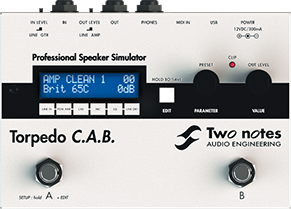
\includegraphics[width=50mm]{torpido.png}
 \end{center}
 \caption{Two notes torpido}
 \label{fig:one}
\end{figure}

インパルス応答の畳み込みによるシミュレートは高い再現度に加えて,インパルス応答の音声データさえ用意できれば,誰でもシミュレートができる手軽さが利点である.しかし,ギター用ひずみエフェクタなどの非線形特性を模倣することは不可能である.

\section{ニューラルネットワークを用いた非線形特性懐疑}
近年,時系列データをニューラルネットワークを用いて処理する研究が注目されている.
音声についても,合成や認識の研究で,成果が報告されており\cite{ninsiki}\cite{gousei},音響フィルター特性のより高精度な再現も,ニューラルネットワークによって可能になると期待が高まっている.

本研究では,非線形特性のシミュレートにおけるニューラルネットワークの有用性を検証するため,ニューラルネットワークを利用したシステムの構築を試みた.

\chapter{音響におけるニューラルネットワーク}
今回の研究では,楽器エフェクタをニューラルネットワークの手法の1つであるLSTM(Long Short-Term Memory)を用いてシミュレートする.
ここでは,RNN(Recurrent Neural Network)の基礎的事項を述べ,その発展的な手法であり,今回使用するLong Short-Term Memoryについて説明する.

\section{再帰的ニューラルネットワーク(RNN: Recurrent Neural Network)}
音声データは(x(1),...x(t),...x(T))というT個のデータが1つの入力データ群となる時系列データである.
時間の概念をニューラルネットワークに取り入れるには,過去の状態をモデル内で保持する必要がある.
RNNは,出力を次のステップに入力として渡すことにより,過去の状態が保持され連続的な情報を利用できる.\cite{RNN}
RNNの構造図を図3.1 に示す.

\begin{figure}[htbp]
 \begin{center}
  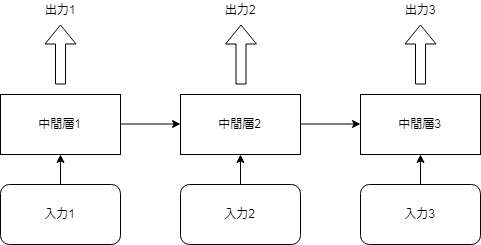
\includegraphics[width=80mm]{RNN.png}
 \end{center}
 \caption{RNN構造図}
 \label{fig:one}
\end{figure}

通常のニューラルネットワークでは,音声や文章,映像などの時系列データを扱うことはできないが,RNN を使うことで中間層が時間方向に展開され,時系列データにも対応できる.

\section{長期依存ニューラルネットワーク(LSTM: Long Short Term Memory)}
RNNは,長期の時間依存性は勾配が消失してしまうことから学習できない.この問題を解決すべく考案されたのがLSTMである.
\newpage

\begin{figure}[htbp]
 \begin{center}
  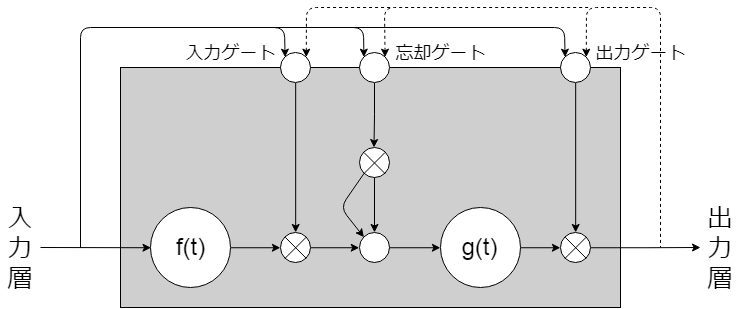
\includegraphics[width=120mm]{LSTM.png}
 \end{center}
 \caption{LSTM構造図}
 \label{fig:one}
\end{figure}

LSTMは,図3.2 のように,通常のニューロンに対し,入力ゲート,出力ゲート,忘却ゲートを追加したユニットを使用する.
入出力ゲートを拡張し,フィードバック機構をつけることで勾配の消失を解消し,長期の学習が可能となる.\cite{RNN}

本研究では,様々な特性のエフェクタに対応できるシミュレータの構築を目的とし,短期依存と長期依存どちらも学習が可能であり,汎用性が高いLSTMを使用する.

\chapter{実験方法}
本章では,LSTMを用いた楽器エフェクタのシミュレータの構築手順,シミュレータの評価方法について記述する.

\section{使用機材}
本実験で使用した機材を表4.1 に示す.
\begin{table}[h]
  \begin{center}
  \caption{使用機材}
  \begin{tabular}{c|cc} \hline
使用機材およびソフト&メーカー,ソフト名&型番 \\ \hline
    オーディオインターフェース&steinberg&UR22 \\
    楽器エフェクター&BOSS&DS-1\\
    音声再生,録音ソフト&Audacity& \\
    学習環境&Google Colaboratory& \\ \hline
  \end{tabular}
 \end{center}
\end{table}

\section{教師データ作成}
学習に使用する教師データを作成した.教師データは,110 msの音声データ(waveファイル)を入力側と出力側をそれぞれ用意し,それら1対を1つのデータセットとして扱った.音声データは-1.0~1.0へ正規化し,1次元ベクトルとして扱う.
\begin{figure}[htbp]
 \begin{minipage}{0.5\hsize}
 \begin{center}
  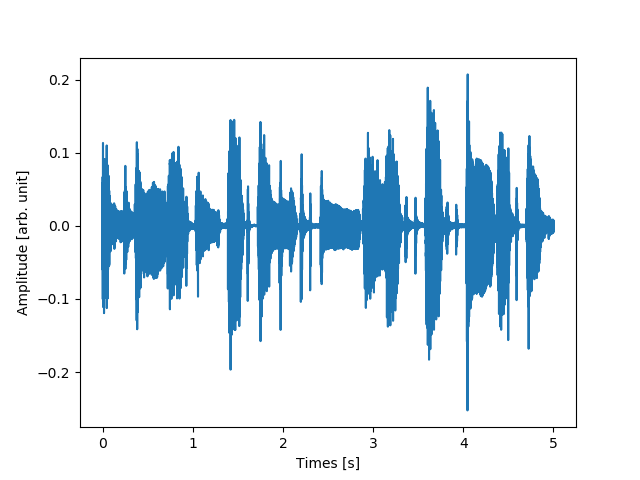
\includegraphics[width=70mm]{train_x0.png}
 \end{center}
 \caption{教師データ入力側例}
 \label{fig:one}
 \end{minipage}
 \begin{minipage}{0.5\hsize}
 \begin{center}
  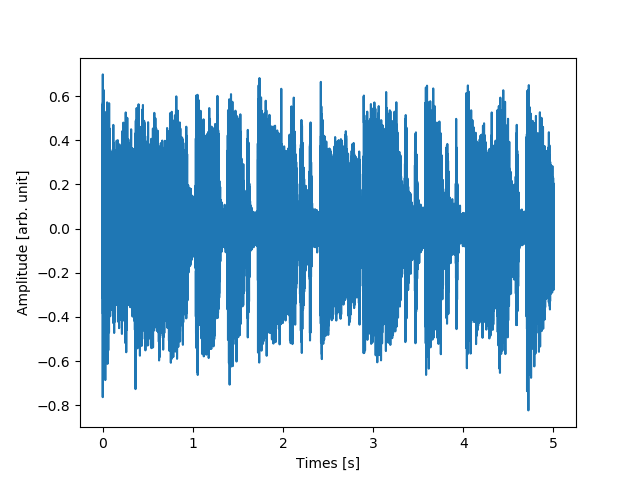
\includegraphics[width=70mm]{train_y0.png}
 \end{center}
 \caption{教師データ出力側例}
 \label{fig:two}
 \end{minipage}
\end{figure}

\subsection{入力側音声データ}
入力側音声データには,ギターの原音を使用した.PCとオーディオインターフェースをUSBケーブル,オーディオインターフェースとギターをアナログオーディオケーブルで結線し,サンプリング周波数を48000 Hz,量子分解能を16 bitに設定して録音を実施した.音域,弦を弾く強さ,単音か和音かを無作為に演奏したデータを50秒分用意した.

\subsection{出力側音声データ}
出力側音声データには,用意した入力側音声データを,ギター用の歪みエフェクタの一種であるBOSS DS-1に通したものを使用する.
オーディオインターフェースを介し,DS-1への入力とDS-1からの出力音声の録音を同時に行った.録音環境の機材構成図を図4.4 に示す.

\begin{figure}[htbp]
 \begin{center}
  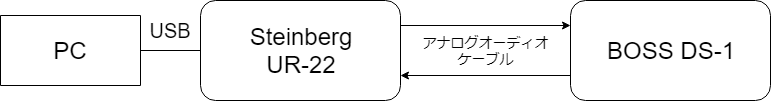
\includegraphics[width=120mm]{env.png}
 \end{center}
 \caption{録音環境}
 \label{fig:one}
\end{figure}

\begin{figure}[htbp]
 \begin{center}
  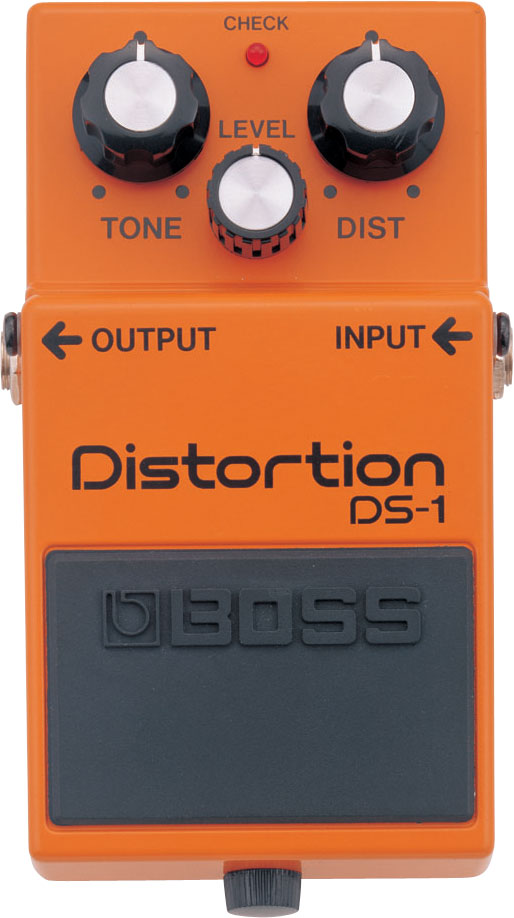
\includegraphics[width=20mm]{ds1.jpg}
 \end{center}
 \caption{BOSS DS-1}
 \label{fig:one}
\end{figure}

DS-1は,DIST,TONE,LEVELの3つのつまみを持つ.つまみの分解能を,1~9の9段階で定義し,DIST,TONEのつまみを表4.2 に示す5パターンの位置に合わせ,データを用意した.LEVELつまみは5で固定し,音量はオーディオインターフェースのプリアンプ部で調整を行い,クリッピングが生じないように設定した.

\begin{table}
  \begin{center}
  \caption{つまみ位置パターン表}
  \begin{tabular}{c|cc} \hline
    パターン名&DISTのつまみ位置&TONEのつまみ位置\\ \hline
    DIST:1&1&5 \\
    DIST:5&5&5 \\
    DIST:9&9&5 \\
    TONE:1&5&1 \\
    TONE:9&5&9 \\ \hline
  \end{tabular}
  \end{center}
\end{table}

\section{学習}

\subsection{モデル構築}
時系列データである音声データを扱うため,LSTMを使用する.モデルの構成は,input units=64,hidden units=64,output units=1とした.
Kerasのモデル可視化機能を使用し,作成したモデル構成図を,図4.5 に示す.

\begin{figure}[htbp]
 \begin{center}
  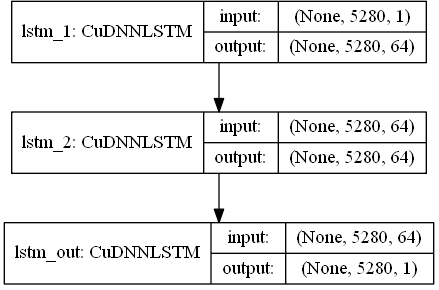
\includegraphics[width=100mm]{model.png}
 \end{center}
 \caption{構築モデル構成図}
 \label{fig:one}
\end{figure}

歪みエフェクタなどの非線形フィルタの出力に100 ms以上の依存情報は無いと考慮し,モデルに入力する教師データの長さは110 msとし,与えられる点数は,48000 Hz $\times$ 110ms $=$ 5280sampleとなる.
LSTMは,入力データ長と同じ長さの出力が得られるが,今回作成したモデルでは,出力された110 msの音声データの末尾10 msを最終出力として使う.推論の際には,入力側音声データを10 msずつずらしながらモデルを適用することで完全な出力を整形する.これにより,出力のすべてが100 msの依存情報を得られる.

\begin{figure}[htbp]
 \begin{center}
  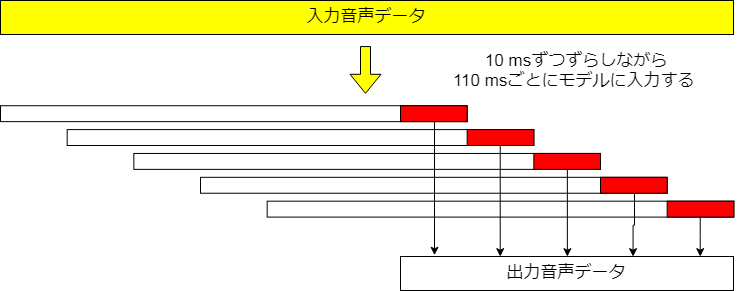
\includegraphics[width=140mm]{suiron.png}
 \end{center}
 \caption{推論イメージ図}
 \label{fig:one}
\end{figure}

\subsection{学習}
ライブラリはTensorflowをバックエンドとしたKerasを使用し,Googleが提供するブラウザ開発環境 Google Colaboratoryにて学習を実行した.
16サンプルを1ステップ,100ステップを1epochとし,100epochの計算を行った.
50 sのデータのうち40 sを学習用データ,10 sをテストデータとし,学習データの損失とテストデータの損失を算出しながら学習を行った.10 sのテストデータにも,
損失関数は,式(4.1) に示した平均二乗誤差(Mean Square Error)を使用した.
\begin{equation}
  MSE(c) = \frac{1}{n}\sum_{i=1}^{n}(x_i-c)^2
\end{equation}
教師データ出力側とモデルの出力の末尾10 msから損失を算出した.

\section{評価実験}
\subsection{出力波形比較}
学習に使用していないギター音声データを,DS-1と実験4.2.2 で得た学習済みモデルに入力し,DS-1から出力された音声データの波形と,モデルから出力された波形を比較した.

\subsection{周波数スペクトル比較}
実験4.3.1 の実験で出力された波形にフーリエ変換処理を行い,DS-1から出力された音声データの波形と,モデルから出力された波形の周波数スペクトルを比較した.

\subsection{推論にかかる時間の測定}
5秒の音源を学習済みモデルに入力し,推論された音源が出力されるまでの時間を測定を行った.

\chapter{結果}
本章では,第4章の実験によって得られた結果について述べる.

\section{学習結果}
用意した5パターンの教師データ,モデルを使用し,100Epochsの計算を行った.計算にはGoogle ColaboratoryのGPUを使用し,100 Epochsの所要時間はおよそ2時間だった.学習の際に算出された,教師データの損失とテストデータの損失,Epochsの関係を図5.1~5.5,表5.1~5.5に示す.
どのパターンも,epochsを重ねるごとに教師データ,テストデータ共に損失は減少しているため,学習により平均二乗誤差を小さくすることに成功している.TONE位置をかえたTONE:1とTONE9のパターンは他と比べ収束が早かった.

\begin{figure}[htbp]
 \begin{center}
  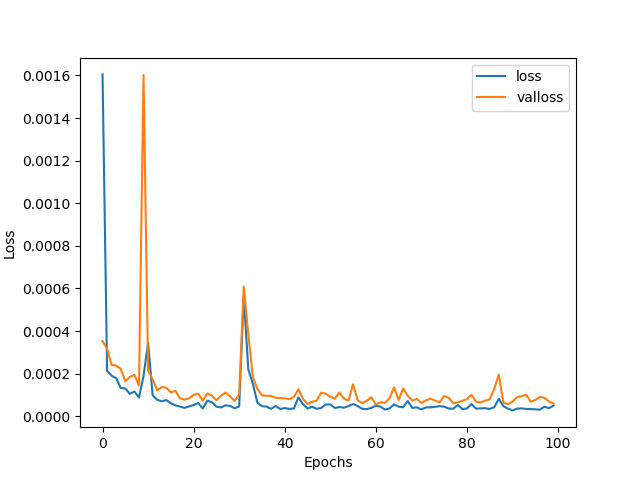
\includegraphics[width=80mm]{gain1_loss_hikaku.png}
 \end{center}
 \caption{DIST:1 教師データ,テストデータの損失比較}
 \label{fig:one}
\end{figure}

\begin{figure}[htbp]
 \begin{center}
  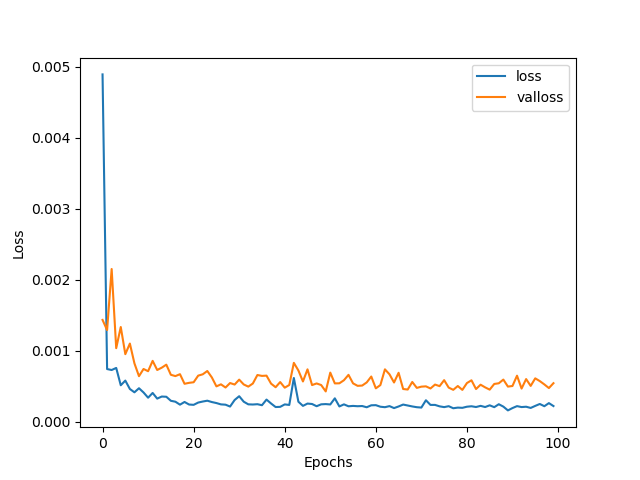
\includegraphics[width=80mm]{gain5_loss_hikaku.png}
 \end{center}
 \caption{DIST:5 教師データ,テストデータの損失比較}
 \label{fig:one}
\end{figure}

\begin{figure}[htbp]
 \begin{center}
  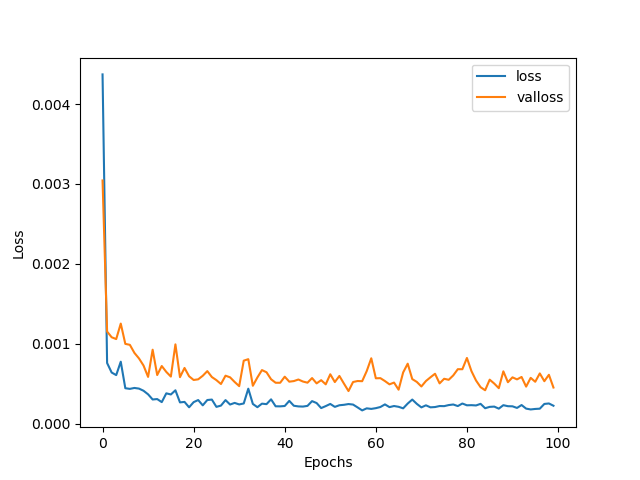
\includegraphics[width=80mm]{gain10_loss_hikaku.png}
 \end{center}
 \caption{DIST:9 教師データ,テストデータの損失比較}
 \label{fig:one}
\end{figure}

\begin{figure}[htbp]
 \begin{center}
  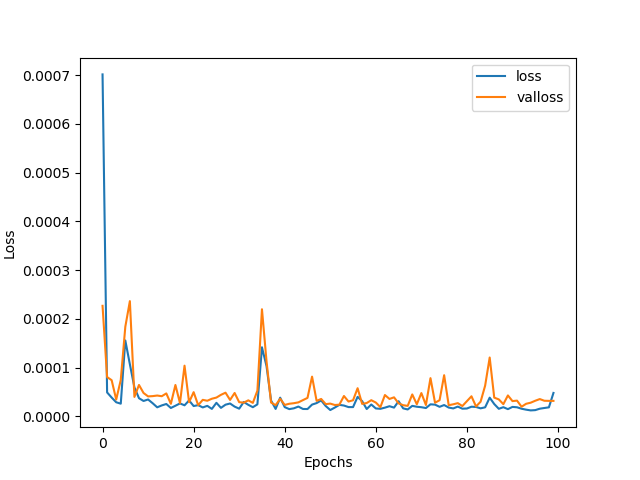
\includegraphics[width=80mm]{tone1_loss_hikaku.png}
 \end{center}
 \caption{TONE:1 教師データ,テストデータの損失比較}
 \label{fig:one}
\end{figure}

\begin{figure}[htbp]
 \begin{center}
  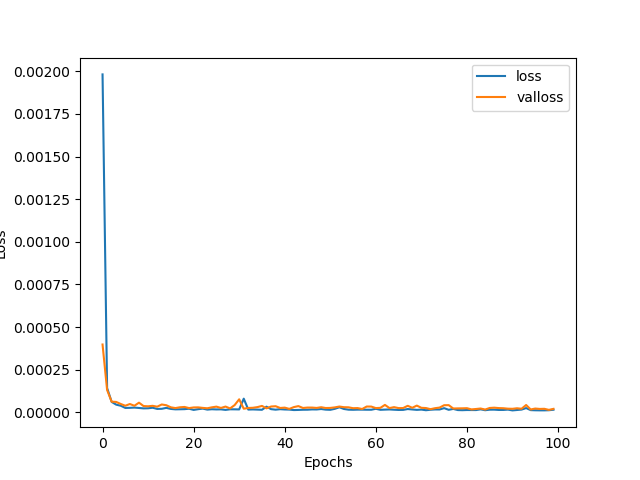
\includegraphics[width=80mm]{tone10_loss_hikaku.png}
 \end{center}
 \caption{TONE:9 教師データ,テストデータの損失比較}
 \label{fig:one}
\end{figure}

\begin{table}
  \begin{center}
  \caption{DIST:1 損失算出結果}
  \begin{tabular}{c|cc} \hline
Step&Train Data Loss&Validation Data Loss \\ \hline
0&0.00160506&0.000352979 \\
%1&0.000213528&0.000317913 \\
2&0.000190245&0.000240705 \\
%3&0.00017848&0.000237906 \\
%4&0.000132364&0.000221933 \\
5&0.000130621&0.000163573 \\
%6&0.000105466&0.000184859 \\
7&0.000115878&0.000194017 \\
%8&8.79E-05&0.00014488 \\
%9&0.000189127&0.001602182 \\
10&0.000345975&0.000215513 \\
%11&9.86E-05&0.000172736 \\
12&7.73E-05&0.000121131 \\
%13&7.00E-05&0.000137317 \\
%14&7.60E-05&0.000134342 \\
15&6.09E-05&0.000112027 \\
%16&5.10E-05&0.000118797 \\
17&4.55E-05&8.47E-05 \\
%18&3.93E-05&7.75E-05 \\
%19&4.62E-05&8.47E-05 \\
20&5.24E-05&0.000100358 \\
%21&6.22E-05&0.000106018 \\
%22&3.65E-05&7.35E-05 \\
%23&7.34E-05&0.000107002 \\
%24&6.59E-05&9.72E-05 \\
25&4.51E-05&7.47E-05 \\
%26&4.13E-05&9.64E-05 \\
%27&5.12E-05&0.000111188 \\
%28&4.85E-05&9.34E-05 \\
%29&3.75E-05&7.17E-05 \\
30&4.58E-05&0.000101449 \\
%31&0.000565476&0.000609122 \\
%32&0.000220356&0.000384264 \\
%33&0.000152444&0.000184091 \\
%34&6.33E-05&0.000127893 \\
%35&4.73E-05&9.80E-05 \\
%36&4.53E-05&9.60E-05 \\
%37&3.47E-05&9.57E-05 \\
%38&4.84E-05&8.67E-05 \\
%39&3.44E-05&8.52E-05 \\
40&3.83E-05&8.37E-05 \\
%41&3.46E-05&8.01E-05 \\
%42&3.60E-05&9.00E-05 \\
%43&8.87E-05&0.000126452 \\
%44&5.68E-05&8.09E-05 \\
%45&3.63E-05&5.76E-05 \\
%46&4.46E-05&6.79E-05 \\
%47&3.50E-05&7.24E-05 \\
%48&3.88E-05&0.000110139 \\
%49&5.54E-05&0.000105566 \\
%50&5.55E-05&9.12E-05 \\
%51&3.89E-05&8.24E-05 \\
%52&4.30E-05&0.000111584 \\
%53&4.03E-05&8.25E-05 \\
%54&4.77E-05&7.39E-05 \\
%55&5.74E-05&0.00015019 \\
%56&4.77E-05&7.57E-05 \\
%57&3.47E-05&6.18E-05 \\
%58&3.35E-05&7.24E-05 \\
%59&3.93E-05&8.95E-05 \\
60&4.90E-05&5.49E-05 \\
%61&4.54E-05&6.57E-05 \\
%62&3.12E-05&6.31E-05 \\
%63&3.67E-05&8.42E-05 \\
%64&5.53E-05&0.000135653 \\
%65&4.51E-05&7.68E-05 \\
%66&4.21E-05&0.000130762 \\
%67&7.15E-05&9.59E-05 \\
%68&3.91E-05&7.35E-05 \\
%69&4.18E-05&8.13E-05 \\
%70&3.20E-05&6.24E-05 \\
%71&4.15E-05&7.45E-05 \\
%72&4.17E-05&8.26E-05 \\
%73&4.44E-05&7.36E-05 \\
%74&4.73E-05&6.51E-05 \\
%75&4.50E-05&9.51E-05 \\
%76&3.66E-05&8.66E-05 \\
%77&3.54E-05&6.10E-05 \\
%78&5.27E-05&6.53E-05 \\
%79&3.38E-05&7.27E-05 \\
80&3.65E-05&8.05E-05 \\
%81&5.75E-05&0.000100877 \\
%82&3.55E-05&6.79E-05 \\
%83&3.69E-05&6.51E-05 \\
%84&3.76E-05&7.29E-05 \\
%85&3.45E-05&7.94E-05 \\
%86&4.25E-05&0.000129144 \\
%87&8.18E-05&0.000195353 \\
%88&4.74E-05&6.41E-05 \\
%89&3.57E-05&5.64E-05 \\
%90&2.74E-05&6.88E-05 \\
%91&3.57E-05&9.00E-05 \\
%92&3.67E-05&9.45E-05 \\
%93&3.45E-05&0.000101003 \\
%94&3.34E-05&6.86E-05 \\
%95&3.27E-05&7.63E-05 \\
%96&3.05E-05&9.04E-05 \\
%97&4.46E-05&8.68E-05 \\
%98&3.78E-05&7.02E-05 \\
99&4.96E-05&5.97E-05 \\ \hline
  \end{tabular}
  \end{center}
\end{table}

\begin{table}
  \begin{center}
  \caption{DIST:5 損失算出結果}
  \begin{tabular}{c|cc} \hline
Step&Train Data Loss&Validation Data Loss \\ \hline
0&0.004889861&0.001435508 \\
%1&0.000744052&0.001292358 \\
2&0.000730644&0.002151775 \\
%3&0.000759727&0.001037813 \\
%4&0.000516023&0.001335694 \\
5&0.000581503&0.000953488 \\
%6&0.000463676&0.001102789 \\
7&0.000416913&0.000824363 \\
%8&0.000473962&0.000643782 \\
%9&0.000414526&0.000745018 \\
10&0.000341153&0.000713648 \\
%11&0.000407701&0.000859346 \\
12&0.000328151&0.000730773 \\
%13&0.00035718&0.000763542 \\
%14&0.000354273&0.000805871 \\
15&0.000297489&0.0006634 \\
%16&0.000284389&0.000644895 \\
17&0.000243047&0.000671774 \\
%18&0.00028088&0.00053688 \\
%19&0.000244971&0.000550054 \\
20&0.000240547&0.000558295 \\
%21&0.000272628&0.000651547 \\
%22&0.000287118&0.0006701 \\
%23&0.000298778&0.000716666 \\
%24&0.000279819&0.000625924 \\
25&0.000265637&0.000500552 \\
%26&0.00024686&0.000529027 \\
%27&0.000242713&0.000484245 \\
%28&0.000216448&0.000547365 \\
%29&0.000308574&0.000525933 \\
30&0.000361822&0.000595148 \\
%31&0.00028465&0.000527179 \\
%32&0.000247558&0.000496814 \\
%33&0.00024506&0.000540644 \\
%34&0.000249534&0.00066011 \\
%35&0.00023539&0.000647761 \\
%36&0.000314367&0.000651432 \\
%37&0.00025952&0.000538898 \\
%38&0.000209661&0.000488401 \\
%39&0.000212282&0.00056086 \\
40&0.000246562&0.000481986 \\
%41&0.0002391&0.000519534 \\
%42&0.000618688&0.000831275 \\
%43&0.000284162&0.00072398 \\
%44&0.00022603&0.000569386 \\
%45&0.000258338&0.000739949 \\
%46&0.000252274&0.000518608 \\
%47&0.000221021&0.000541543 \\
%48&0.000247741&0.000519179 \\
%49&0.000251099&0.00042931 \\
%50&0.000245777&0.000693919 \\
%51&0.000331987&0.000542177 \\
%52&0.000217924&0.000543535 \\
%53&0.000247419&0.000586915 \\
%54&0.000220274&0.000662473 \\
%55&0.000225418&0.000542753 \\
%56&0.000221106&0.000507839 \\
%57&0.000223819&0.000511765 \\
%58&0.000206551&0.000555992 \\
%59&0.000234044&0.000638897 \\
60&0.00023607&0.00047275 \\
%61&0.000214041&0.000518529 \\
%62&0.000207452&0.000740037 \\
%63&0.000222599&0.000669925 \\
%64&0.000194841&0.000554937 \\
%65&0.000217739&0.000691593 \\
%66&0.000244407&0.000463404 \\
%67&0.000231235&0.000455803 \\
%68&0.000217875&0.000562175 \\
%69&0.000207241&0.000479158 \\
%70&0.000202159&0.000496308 \\
%71&0.000305013&0.000500735 \\
%72&0.00023932&0.000470841 \\
%73&0.000239582&0.000525681 \\
%74&0.000219321&0.000503637 \\
%75&0.000208494&0.000587894 \\
%76&0.000221513&0.000482938 \\
%77&0.000192633&0.000451671 \\
%78&0.000201512&0.000505388 \\
%79&0.000198546&0.000450816 \\
80&0.000214268&0.000546847 \\
%81&0.000220396&0.000585774 \\
%82&0.000209849&0.000462698 \\
%83&0.000226151&0.000523901 \\
%84&0.000209637&0.000486445 \\
%85&0.000233725&0.000454348 \\
%86&0.000207779&0.000534305 \\
%87&0.000249129&0.000543835 \\
%88&0.000215401&0.000595839 \\
%89&0.000162287&0.000497318 \\
%90&0.000195022&0.000505558 \\
%91&0.000222369&0.000650684 \\
%92&0.000209206&0.000469517 \\
%93&0.000213904&0.000603006 \\
%94&0.000196948&0.000506937 \\
%95&0.000225688&0.000613343 \\
%96&0.000252643&0.00057468 \\
%97&0.000221213&0.000527929 \\
%98&0.000264768&0.000476609 \\
99&0.000223447&0.000545185 \\ \hline
  \end{tabular}
  \end{center}
\end{table}

\begin{table}
  \begin{center}
  \caption{DIST:9 損失算出結果}
  \begin{tabular}{c|cc} \hline
Step&Train Data Loss&Validation Data Loss \\ \hline
0&0.004371066&0.003043697 \\
%1&0.000759486&0.001153236 \\
2&0.000640299&0.00108158 \\
%3&0.0006079&0.001058804 \\
%4&0.000775743&0.001252678 \\
5&0.00044388&0.000998803 \\
%6&0.000435707&0.000986739 \\
7&0.000447211&0.000885568 \\
%8&0.000439035&0.000816686 \\
%9&0.000412046&0.000727394 \\
10&0.000367349&0.000585502 \\
%11&0.000302804&0.000925947 \\
12&0.000308004&0.000608787 \\
%13&0.000269993&0.00072153 \\
%14&0.000379837&0.000647763 \\
15&0.000365632&0.000589616 \\
%16&0.000417786&0.000992585 \\
17&0.00026646&0.000582271 \\
%18&0.000272529&0.000697525 \\
%19&0.000205124&0.000593352 \\
20&0.000269611&0.000546894 \\
%21&0.000295828&0.000555101 \\
%22&0.000229603&0.000599482 \\
%23&0.000296179&0.000657793 \\
%24&0.000301725&0.000583811 \\
25&0.000210636&0.000544931 \\
%26&0.000226497&0.000496407 \\
%27&0.000295127&0.000600613 \\
%28&0.000239622&0.000580198 \\
%29&0.000260026&0.000522202 \\
30&0.000240948&0.000469696 \\
%31&0.000253004&0.000788571 \\
%32&0.000437932&0.000807393 \\
%33&0.000247104&0.000474404 \\
%34&0.000206442&0.000578834 \\
%35&0.000250729&0.000670884 \\
%36&0.000244497&0.000643456 \\
%37&0.000304898&0.000556043 \\
%38&0.000217728&0.000512277 \\
%39&0.000216928&0.000511966 \\
40&0.000221378&0.0005882 \\
%41&0.000285384&0.000525731 \\
%42&0.000224457&0.000533225 \\
%43&0.000216155&0.00055278 \\
%44&0.000214125&0.000527411 \\
%45&0.000222938&0.000513057 \\
%46&0.000282341&0.000570891 \\
%47&0.0002583&0.000504511 \\
%48&0.000195442&0.000544505 \\
%49&0.000219991&0.00049247 \\
%50&0.000247146&0.000618363 \\
%51&0.000210352&0.000520906 \\
%52&0.00023072&0.000597587 \\
%53&0.000236277&0.000501816 \\
%54&0.000245679&0.000408237 \\
%55&0.000239251&0.000521492 \\
%56&0.00020355&0.000533951 \\
%57&0.000166262&0.000531644 \\
%58&0.000191958&0.000658119 \\
%59&0.000185058&0.000818428 \\
60&0.000194305&0.000568074 \\
%61&0.000208612&0.00056979 \\
%62&0.000241436&0.00053354 \\
%63&0.000207308&0.000492455 \\
%64&0.000221103&0.000514421 \\
%65&0.000211333&0.00042526 \\
%66&0.000192082&0.000641374 \\
%67&0.000251961&0.000750981 \\
%68&0.000301935&0.000558112 \\
%69&0.000248095&0.000522636 \\
%70&0.000204014&0.000465629 \\
%71&0.000229827&0.000533853 \\
%72&0.000204647&0.000580661 \\
%73&0.000208323&0.000624949 \\
%74&0.000220868&0.000504471 \\
%75&0.000219498&0.000562008 \\
%76&0.000232896&0.000549256 \\
%77&0.00024018&0.000604114 \\
%78&0.000220515&0.00068188 \\
%79&0.000252392&0.00068151 \\
80&0.00023004&0.000822419 \\
%81&0.000231819&0.000657189 \\
%82&0.000228214&0.000540706 \\
%83&0.000248164&0.000456805 \\
%84&0.000193526&0.000418304 \\
%85&0.000210376&0.000550775 \\
%86&0.000213836&0.000502167 \\
%87&0.000188316&0.000444256 \\
%88&0.000231664&0.000655027 \\
%89&0.000218846&0.000518907 \\
%90&0.000217386&0.000579928 \\
%91&0.000197123&0.000554434 \\
%92&0.000233412&0.000584695 \\
%93&0.00018866&0.000463876 \\
%94&0.00017825&0.000573682 \\
%95&0.000184455&0.000524485 \\
%96&0.000187724&0.000629065 \\
%97&0.000247089&0.000531696 \\
%98&0.000253038&0.00061189 \\
99&0.000224676&0.000452522 \\ \hline
  \end{tabular}
  \end{center}
\end{table}

\begin{table}
  \begin{center}
  \caption{TONE:1 損失算出結果}
  \begin{tabular}{c|cc} \hline
Step&Train Data Loss&Validation Data Loss \\ \hline
0&0.0007013146532699466&0.00022688592434860766 \\
3&2.9152513889130205e-05&3.4760440030368045e-05 \\
5&0.00015583523781970143&0.0001840399781940505 \\
7&5.957199391559698e-05&4.0086764784064144e-05 \\
10&3.485469278530218e-05&4.1204581066267565e-05 \\
12&1.881301614048425e-05&4.296326369512826e-05 \\
15&1.746028101479169e-05&2.6004530809586868e-05 \\
17&2.679046883713454e-05&2.7524380129761994e-05 \\
20&2.1427540559670888e-05&4.987289139535278e-05 \\
25&2.80227013718104e-05&3.8780399336246774e-05 \\
30&1.6034053260227665e-05&2.935692282335367e-05 \\
40&1.9162522221449763e-05&2.3683454855927266e-05 \\
60&1.6490608686581254e-05&2.8594282412086613e-05 \\
80&1.637919012864586e-05&3.145473965560086e-05 \\
99&4.827618977287784e-05&3.2005205866880715e-05 \\ \hline
  \end{tabular}
  \end{center}
\end{table}

\begin{table}
  \begin{center}
  \caption{TONE:9 損失算出結果}
  \begin{tabular}{c|cc} \hline
Step&Train Data Loss&Validation Data Loss \\ \hline
0&0.001982149202376604&0.0003975852159783244 \\
2&6.085033965064213e-05&6.210451101651415e-05 \\
5&2.53476628131466e-05&3.8263049646047875e-05 \\
7&2.7467322070151567e-05&3.814345836872235e-05 \\
10&2.3372555006062612e-05&3.508674126351252e-05 \\
12&1.9653545678011142e-05&3.275131530244835e-05 \\
15&1.9577020793803968e-05&2.8969265258638188e-05 \\
17&1.7629268768359907e-05&2.931749440904241e-05 \\
20&1.3814149497193284e-05&2.8302541977609508e-05 \\
25&1.664215415075887e-05&3.297820148873143e-05 \\
30&1.6657786545692943e-05&7.608786108903587e-05 \\
40&1.6345087715308182e-05&2.7229476472712122e-05 \\
60&2.03736090043094e-05&2.4513718017260544e-05 \\
80&1.3250346455606632e-05&2.3967377273947932e-05 \\
99&1.4830713553237729e-05&1.9955643438152038e-05 \\ \hline
  \end{tabular}
  \end{center}
\end{table}

\section{出力波形}
実験5.1 の結果から,最もvalidationlossが低くなったEpochsのモデルを用いて,推論し,教師データとの比較を行った.推論の際,入力データは学習に使用していない音源を使用した.
5秒間演奏した音源を2つ用意し,それぞれ0.00~0.02 s,2.00~2.02,4.00~4.02の3箇所を拡大し,教師データとモデルの出力を比較した.
出力波形を図5,6~5.10に示す.
どのパターンのモデルも,概ね教師信号に追従した波形を出力していることがわかる.
DIST:5,9はDIST:1,TONE:1,TONE:9より教師データとモデルの出力の波形のずれが大きくなる傾向にある.

%DIST1
\begin{figure}[htbp]
 \begin{minipage}{0.5\hsize}
 \begin{center}
  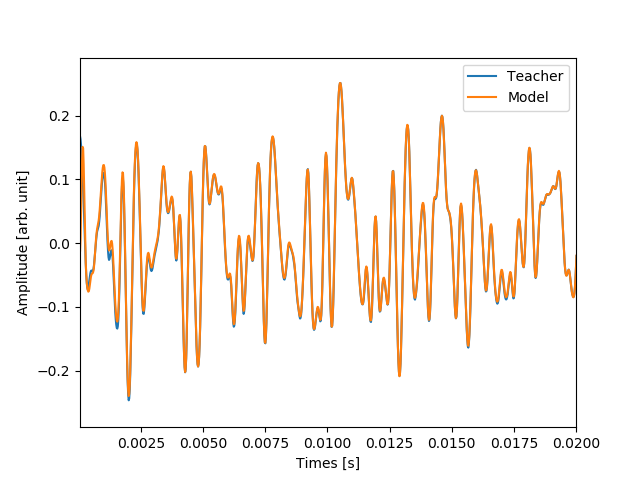
\includegraphics[width=90mm]{gain1_output_hikaku.png}
 \end{center}
 \subcaption{音源1 0.00~0.02 s}
 \label{fig:one}
 \end{minipage}
 \begin{minipage}{0.5\hsize}
 \begin{center}
  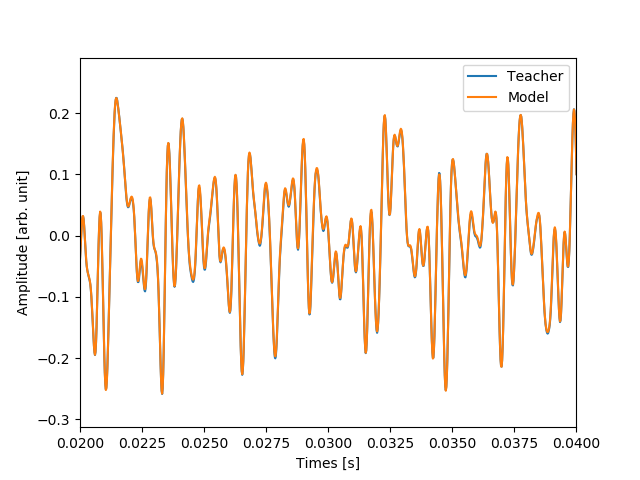
\includegraphics[width=90mm]{gain1_output_hikaku2.png}
 \end{center}
 \subcaption{音源1 2.00~2.02 s}
 \label{fig:two}
 \end{minipage}
 \begin{minipage}{0.5\hsize}
 \begin{center}
  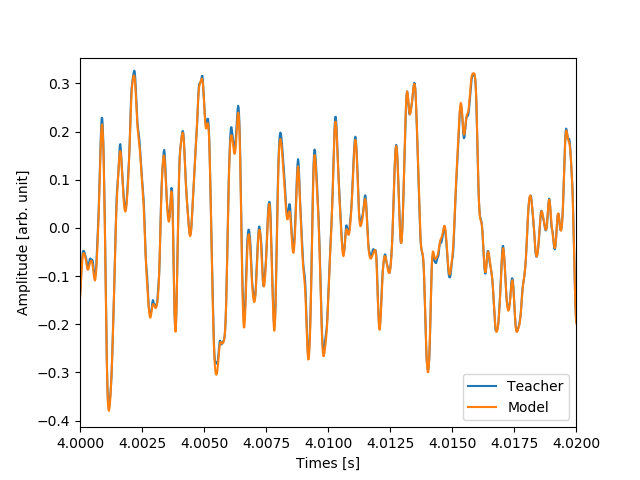
\includegraphics[width=90mm]{gain1_output_hikaku3.png}
 \end{center}
 \subcaption{音源1 4.00~4.02 s}
 \label{fig:one}
 \end{minipage}
 \begin{minipage}{0.5\hsize}
 \begin{center}
  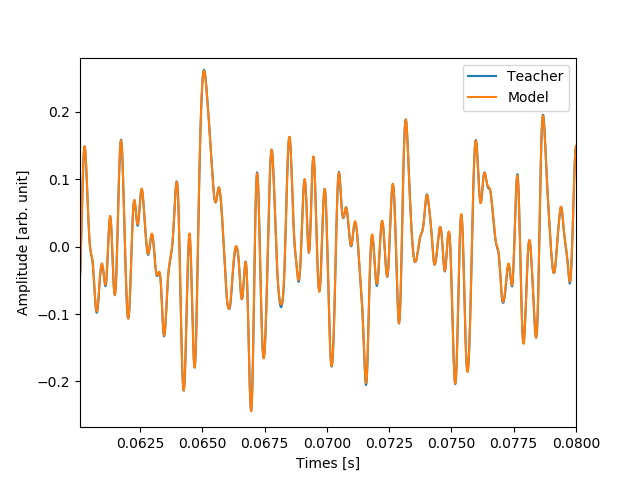
\includegraphics[width=90mm]{gain1_output_hikaku4.png}
 \end{center}
 \subcaption{音源2 0.00~0.02 s}
 \label{fig:two}
 \end{minipage}
 \begin{minipage}{0.5\hsize}
 \begin{center}
  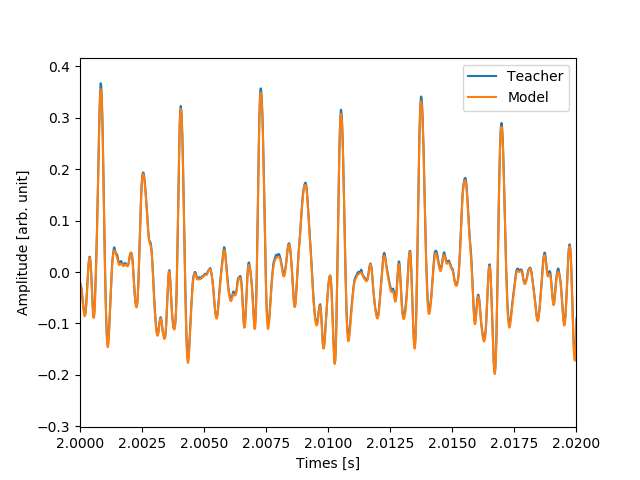
\includegraphics[width=90mm]{gain1_output_hikaku5.png}
 \end{center}
 \subcaption{音源2 2.00~2.02 s}
 \label{fig:one}
 \end{minipage}
 \begin{minipage}{0.5\hsize}
 \begin{center}
  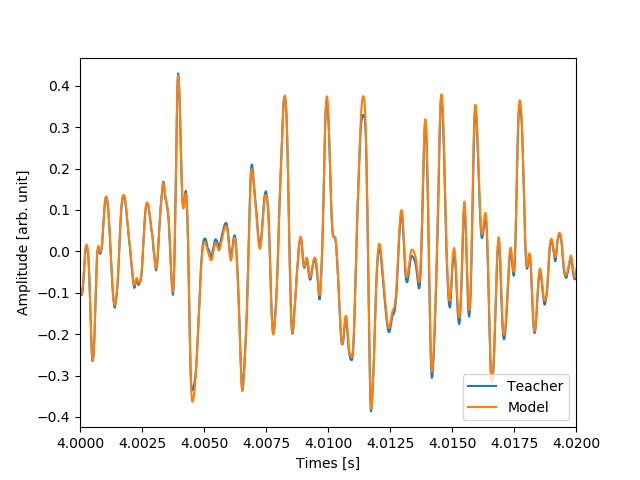
\includegraphics[width=90mm]{gain1_output_hikaku6.png}
 \end{center}
 \subcaption{音源2 4.00~4.02 s}
 \label{fig:two}
 \end{minipage}
 \caption{DIST:1 波形拡大比較}
\end{figure}

%dist5
\begin{figure}[htbp]
 \begin{minipage}{0.5\hsize}
 \begin{center}
  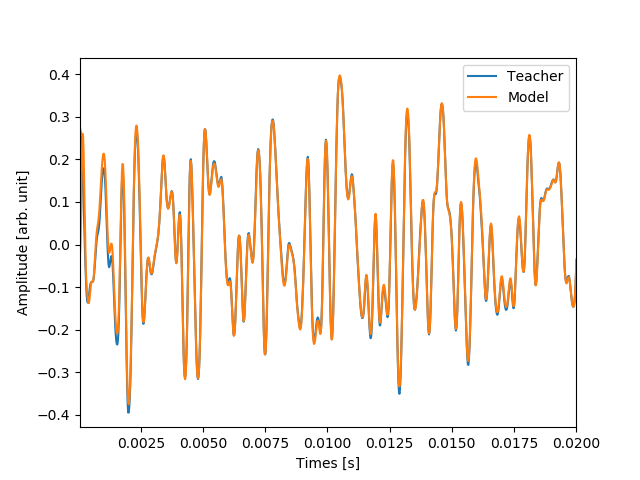
\includegraphics[width=90mm]{gain5_output_hikaku.png}
 \end{center}
 \subcaption{音源1 0.00~0.02 s}
 \label{fig:one}
 \end{minipage}
 \begin{minipage}{0.5\hsize}
 \begin{center}
  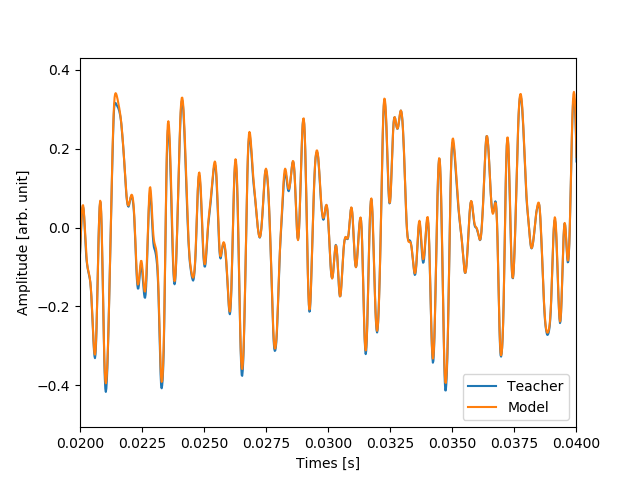
\includegraphics[width=90mm]{gain5_output_hikaku2.png}
 \end{center}
 \subcaption{音源1 2.00~2.02 s}
 \label{fig:two}
 \end{minipage}
 \begin{minipage}{0.5\hsize}
 \begin{center}
  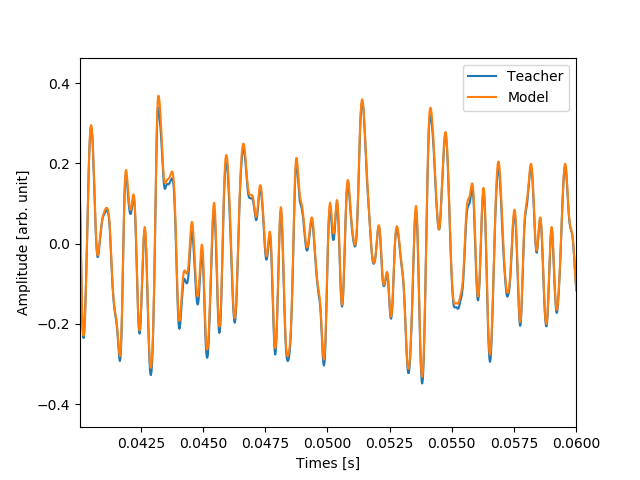
\includegraphics[width=90mm]{gain5_output_hikaku3.png}
 \end{center}
 \subcaption{音源1 4.00~4.02 s}
 \label{fig:one}
 \end{minipage}
 \begin{minipage}{0.5\hsize}
 \begin{center}
  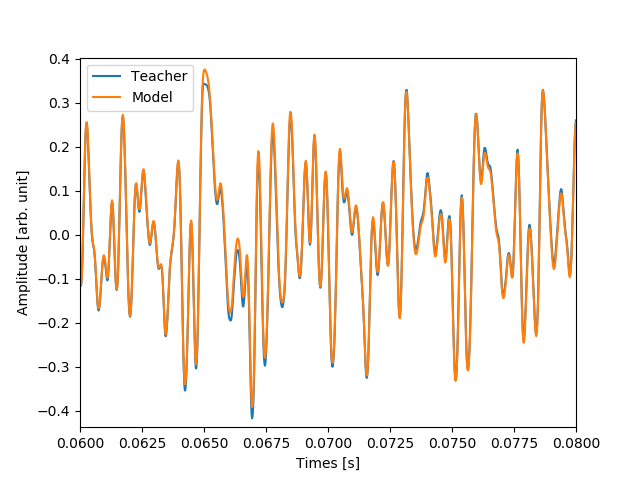
\includegraphics[width=90mm]{gain5_output_hikaku4.png}
 \end{center}
 \subcaption{音源2 0.00~0.02 s}
 \label{fig:two}
 \end{minipage}
 \begin{minipage}{0.5\hsize}
 \begin{center}
  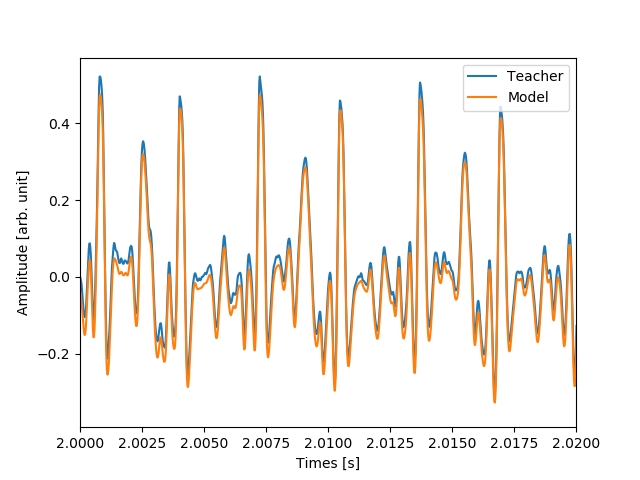
\includegraphics[width=90mm]{gain5_output_hikaku5.png}
 \end{center}
 \subcaption{音源2 2.00~2.02 s}
 \label{fig:one}
 \end{minipage}
 \begin{minipage}{0.5\hsize}
 \begin{center}
  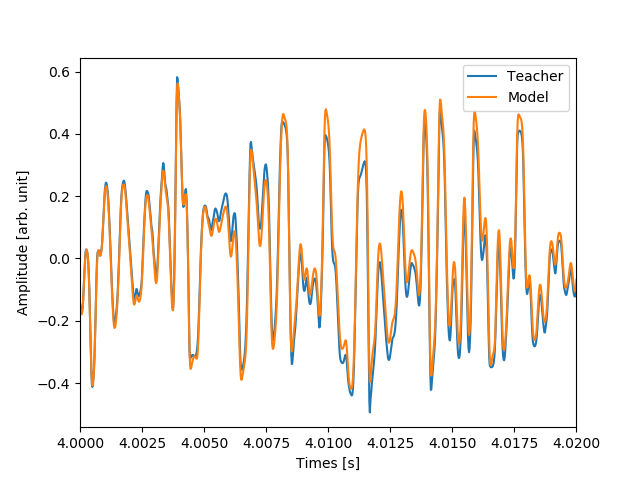
\includegraphics[width=90mm]{gain5_output_hikaku6.png}
 \end{center}
 \subcaption{音源2 4.00~4.02 s}
 \label{fig:two}
 \end{minipage}
 \caption{DIST:5 波形拡大比較}
\end{figure}

\newpage
%DIST10
\begin{figure}[htbp]
 \begin{minipage}{0.5\hsize}
 \begin{center}
  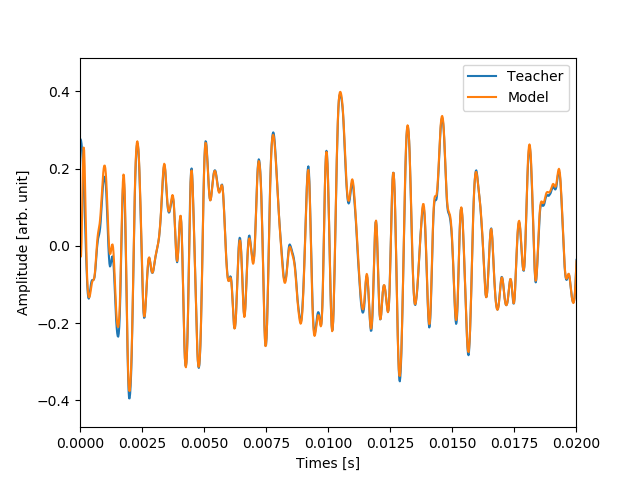
\includegraphics[width=90mm]{gain10_output_hikaku.png}
 \end{center}
 \subcaption{音源1 0.00~0.02 s}
 \label{fig:one}
 \end{minipage}
 \begin{minipage}{0.5\hsize}
 \begin{center}
  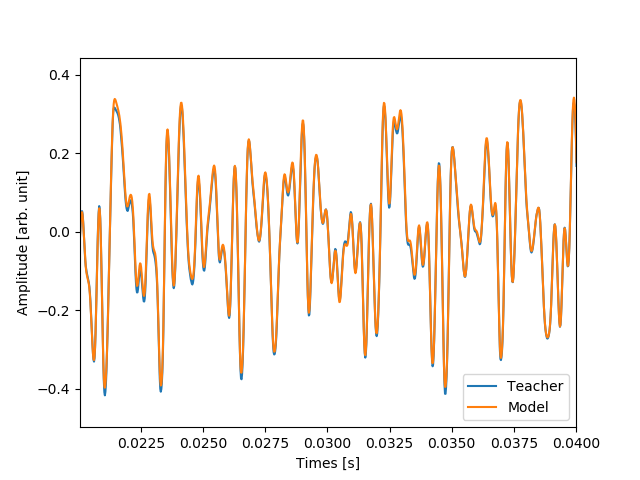
\includegraphics[width=90mm]{gain10_output_hikaku2.png}
 \end{center}
 \subcaption{音源1 2.00~2.02 s}
 \label{fig:two}
 \end{minipage}
 \begin{minipage}{0.5\hsize}
 \begin{center}
  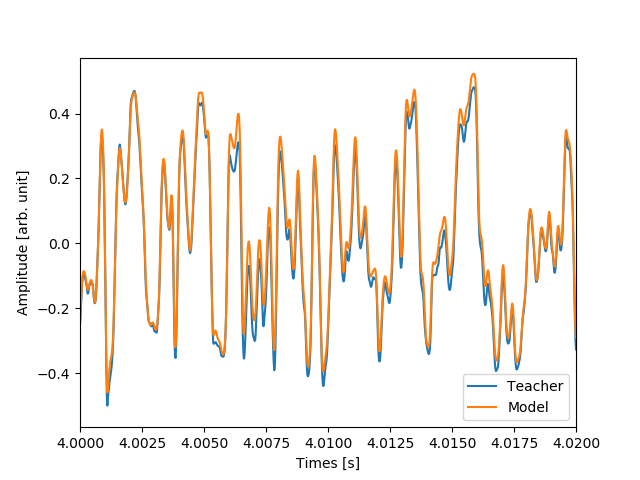
\includegraphics[width=90mm]{gain10_output_hikaku3.png}
 \end{center}
 \subcaption{音源1 4.00~4.02 s}
 \label{fig:one}
 \end{minipage}
 \begin{minipage}{0.5\hsize}
 \begin{center}
  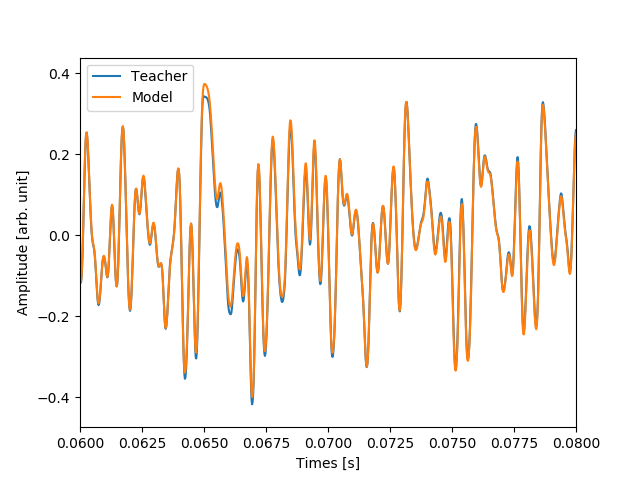
\includegraphics[width=90mm]{gain10_output_hikaku4.png}
 \end{center}
 \subcaption{音源2 0.00~0.02 s}
 \label{fig:two}
 \end{minipage}
 \begin{minipage}{0.5\hsize}
 \begin{center}
  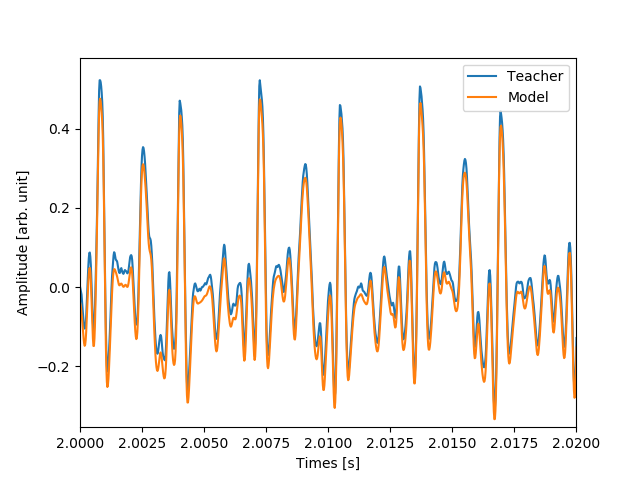
\includegraphics[width=90mm]{gain10_output_hikaku5.png}
 \end{center}
 \subcaption{音源2 2.00~2.02 s}
 \label{fig:one}
 \end{minipage}
 \begin{minipage}{0.5\hsize}
 \begin{center}
  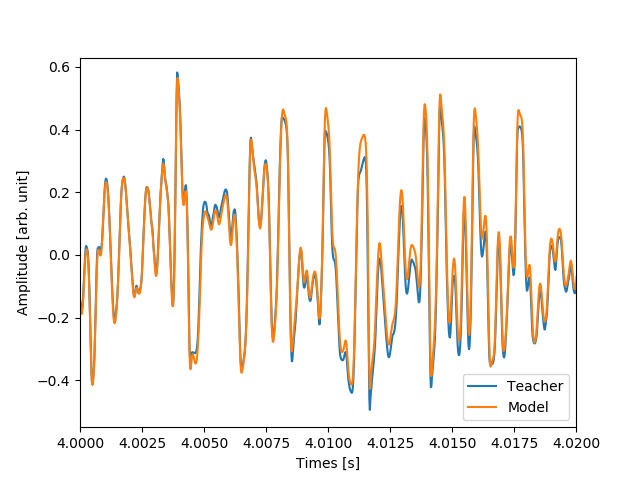
\includegraphics[width=90mm]{gain10_output_hikaku6.png}
 \end{center}
 \subcaption{音源2 4.00~4.02 s}
 \label{fig:two}
 \end{minipage}
 \caption{DIST:9 波形拡大比較}
\end{figure}

%TONE1
\begin{figure}[htbp]
 \begin{minipage}{0.5\hsize}
 \begin{center}
  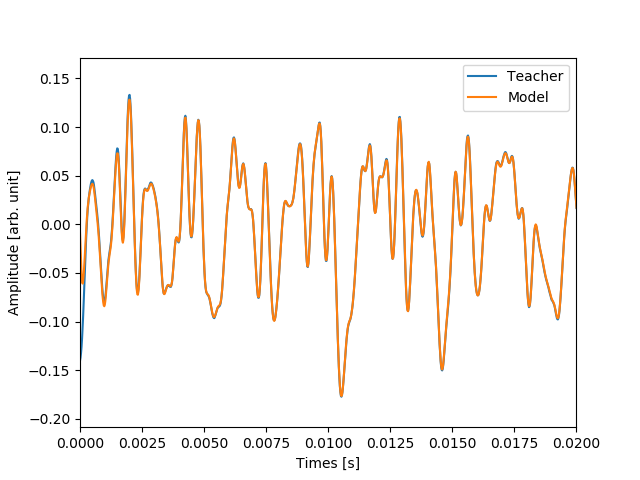
\includegraphics[width=90mm]{tone1_output_hikaku.png}
 \end{center}
 \subcaption{音源1 0.00~0.02 s}
 \label{fig:one}
 \end{minipage}
 \begin{minipage}{0.5\hsize}
 \begin{center}
  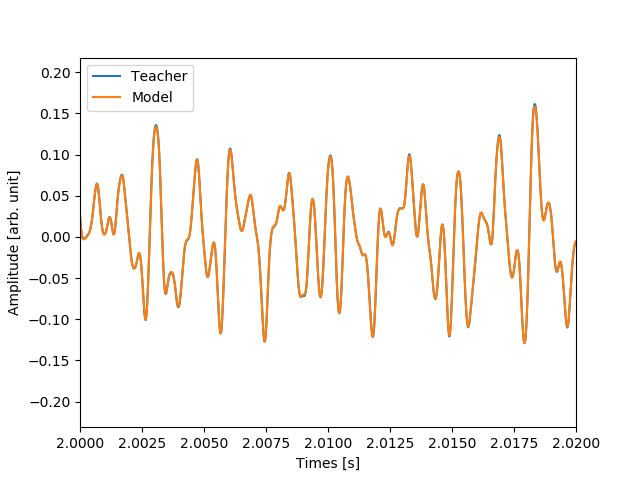
\includegraphics[width=90mm]{tone1_output_hikaku2.png}
 \end{center}
 \subcaption{音源1 2.00~2.02 s}
 \label{fig:two}
 \end{minipage}
 \begin{minipage}{0.5\hsize}
 \begin{center}
  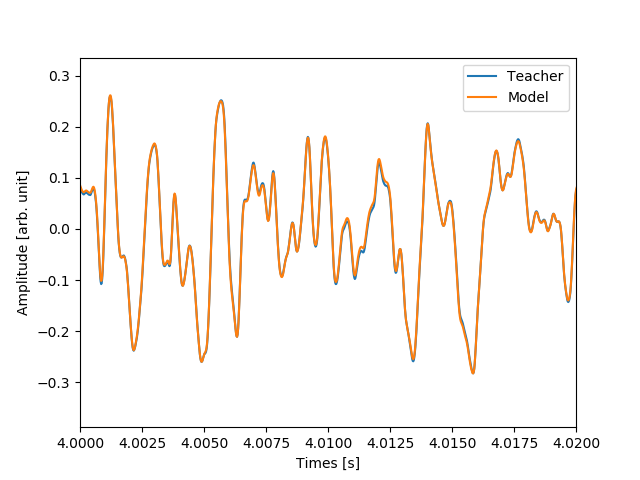
\includegraphics[width=90mm]{tone1_output_hikaku3.png}
 \end{center}
 \subcaption{音源1 4.00~4.02 s}
 \label{fig:one}
 \end{minipage}
 \begin{minipage}{0.5\hsize}
 \begin{center}
  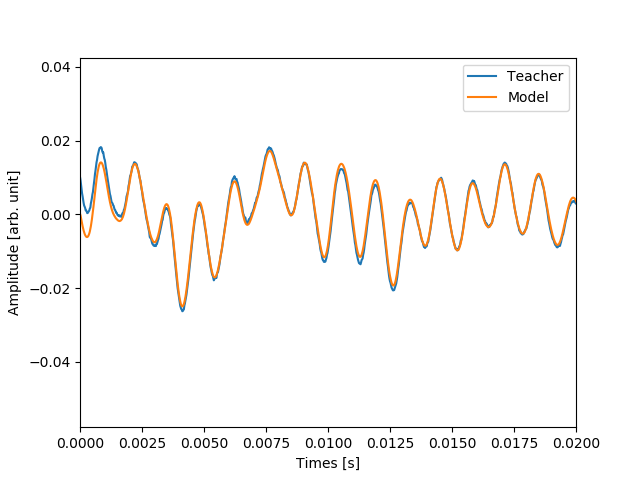
\includegraphics[width=90mm]{tone1_output_hikaku4.png}
 \end{center}
 \subcaption{音源2 0.00~0.02 s}
 \label{fig:two}
 \end{minipage}
 \begin{minipage}{0.5\hsize}
 \begin{center}
  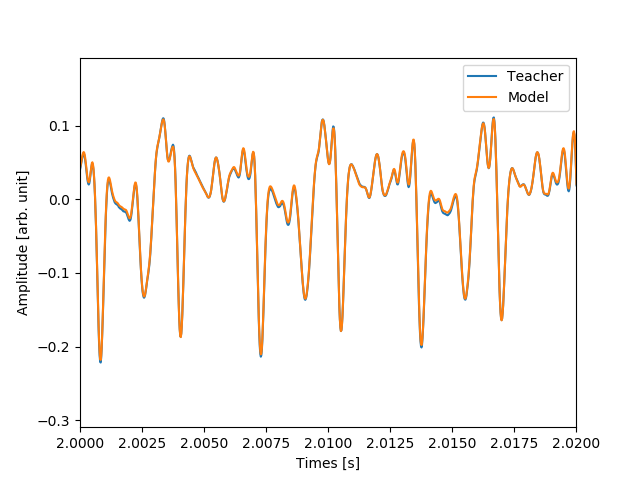
\includegraphics[width=90mm]{tone1_output_hikaku5.png}
 \end{center}
 \subcaption{音源2 2.00~2.02 s}
 \label{fig:one}
 \end{minipage}
 \begin{minipage}{0.5\hsize}
 \begin{center}
  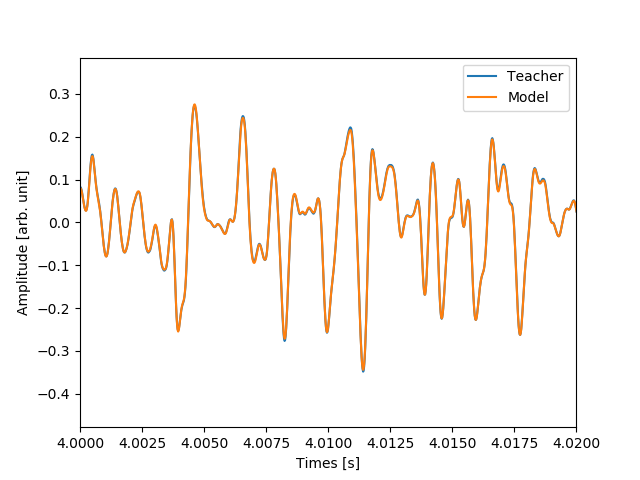
\includegraphics[width=90mm]{tone1_output_hikaku6.png}
 \end{center}
 \subcaption{音源2 4.00~4.02 s}
 \label{fig:two}
 \end{minipage}
 \caption{TONE:1 波形拡大比較}
\end{figure}

%TONE10
\begin{figure}[htbp]
 \begin{minipage}{0.5\hsize}
 \begin{center}
  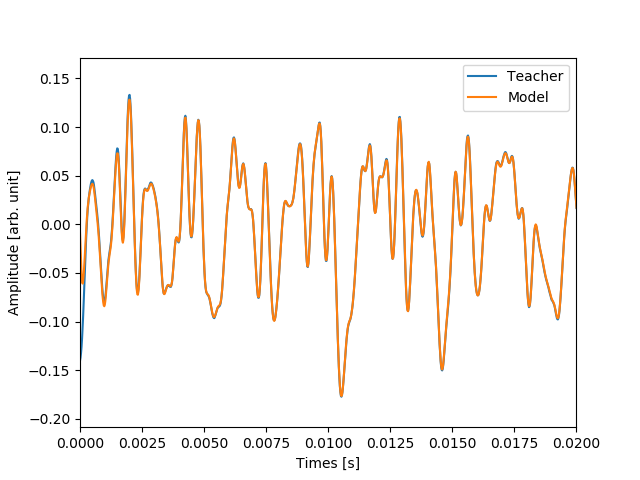
\includegraphics[width=90mm]{tone1_output_hikaku.png}
 \end{center}
 \subcaption{音源1 0.00~0.02 s}
 \label{fig:one}
 \end{minipage}
 \begin{minipage}{0.5\hsize}
 \begin{center}
  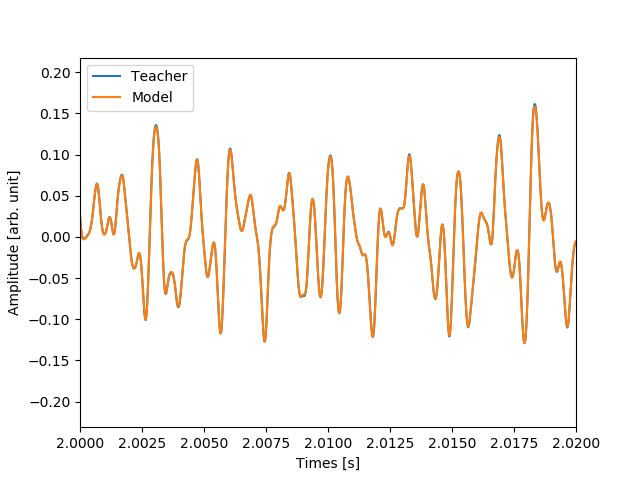
\includegraphics[width=90mm]{tone1_output_hikaku2.png}
 \end{center}
 \subcaption{音源1 2.00~2.02 s}
 \label{fig:two}
 \end{minipage}
 \begin{minipage}{0.5\hsize}
 \begin{center}
  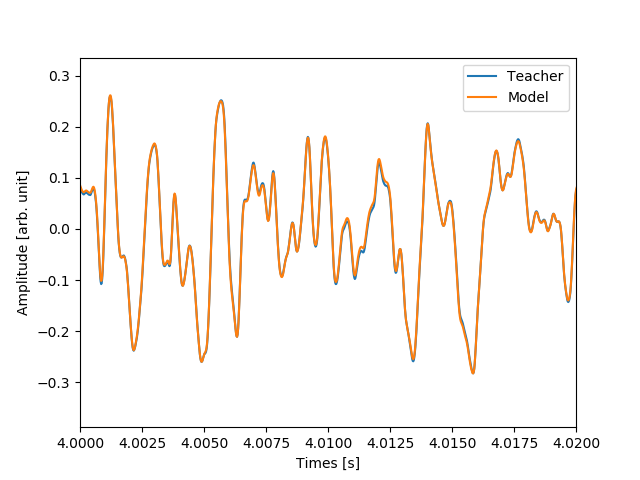
\includegraphics[width=90mm]{tone1_output_hikaku3.png}
 \end{center}
 \subcaption{音源1 4.00~4.02 s}
 \label{fig:one}
 \end{minipage}
 \begin{minipage}{0.5\hsize}
 \begin{center}
  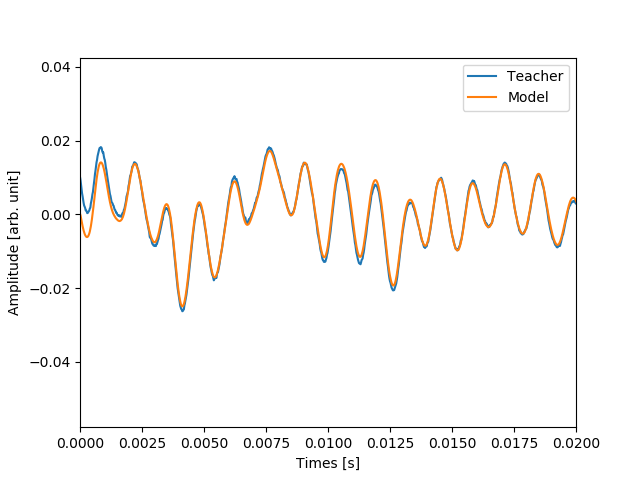
\includegraphics[width=90mm]{tone1_output_hikaku4.png}
 \end{center}
 \subcaption{音源2 0.00~0.02 s}
 \label{fig:two}
 \end{minipage}
 \begin{minipage}{0.5\hsize}
 \begin{center}
  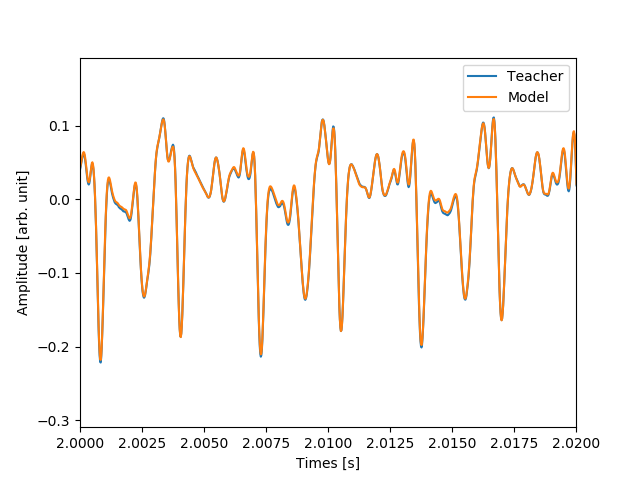
\includegraphics[width=90mm]{tone1_output_hikaku5.png}
 \end{center}
 \subcaption{音源2 2.00~2.02 s}
 \label{fig:one}
 \end{minipage}
 \begin{minipage}{0.5\hsize}
 \begin{center}
  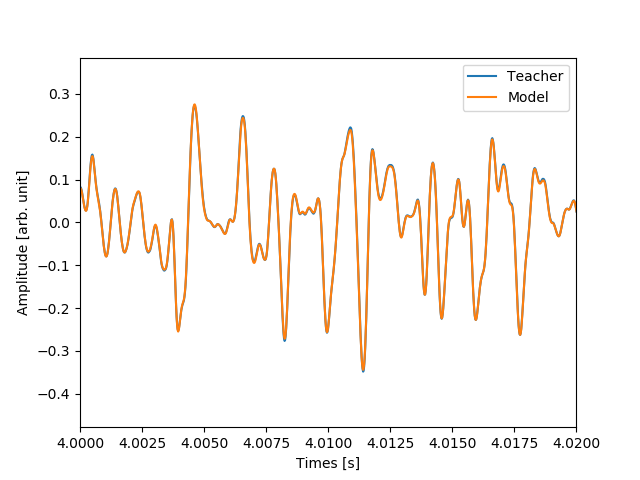
\includegraphics[width=90mm]{tone1_output_hikaku6.png}
 \end{center}
 \subcaption{音源2 4.00~4.02 s}
 \label{fig:two}
 \end{minipage}
 \caption{TONE:9 波形拡大比較}
\end{figure}

\clearpage

\section{スペクトル分析}
実験5.2で使用した音源をモデルに入力したときの出力と教師データにフーリエ変換処理を行い,比較した.窓関数は矩形窓を使用した.解析結果を図5.7,5.8,5.9に示す.
どのパターンのモデルも,低音域は高い最限度を実現しているが,6000 Hz以降の再現度が著しく低下していることがわかる.

\begin{figure}[htbp]
 \begin{minipage}{0.5\hsize}
 \begin{center}
  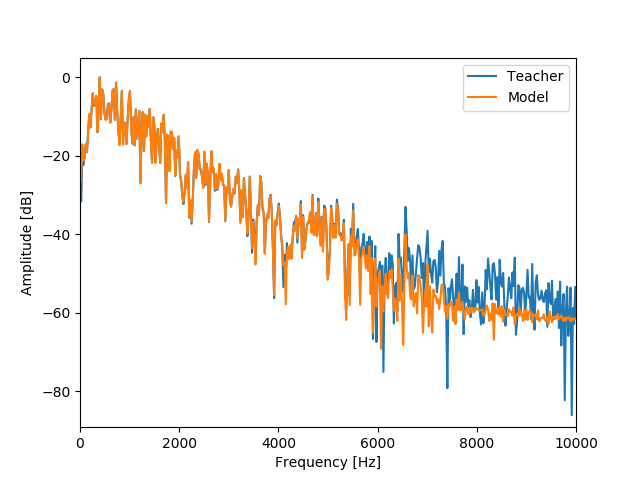
\includegraphics[width=90mm]{gain1_fft_hikaku.png}
 \end{center}
   \subcaption{音声1}
 \label{fig:one}
 \end{minipage}
 \begin{minipage}{0.5\hsize}
 \begin{center}
  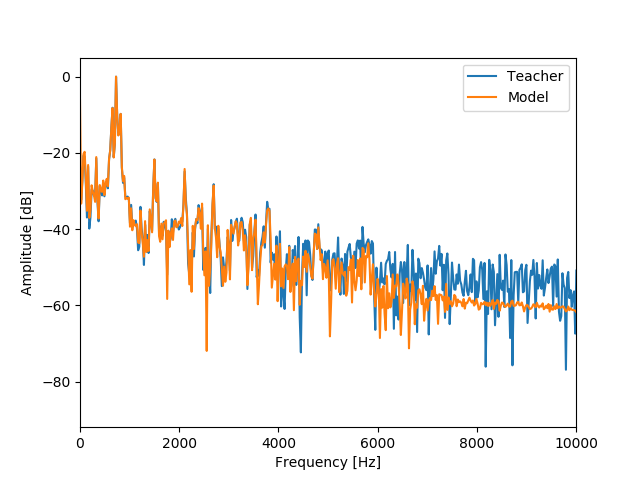
\includegraphics[width=90mm]{gain1_fft_hikaku2.png}
 \end{center}
   \subcaption{音声2}
 \label{fig:two}
 \end{minipage}
 \caption{DIST:1 教師データ,モデル出力周波数スペクトル比較}
\end{figure}

\begin{figure}[htbp]
 \begin{minipage}{0.5\hsize}
 \begin{center}
  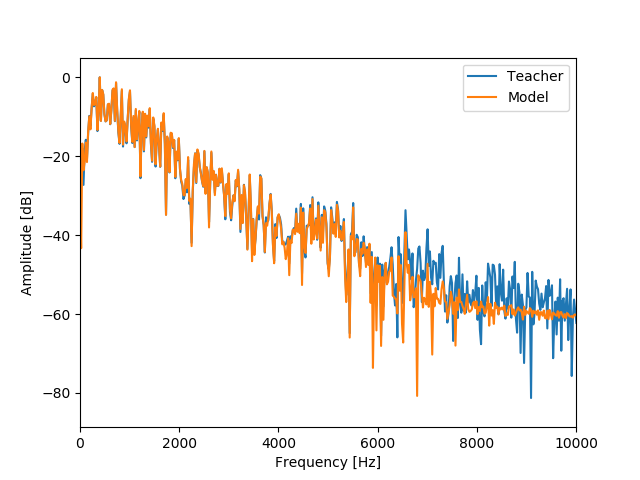
\includegraphics[width=90mm]{gain5_fft_hikaku.png}
 \end{center}
   \subcaption{音声1}
 \label{fig:one}
 \end{minipage}
 \begin{minipage}{0.5\hsize}
 \begin{center}
  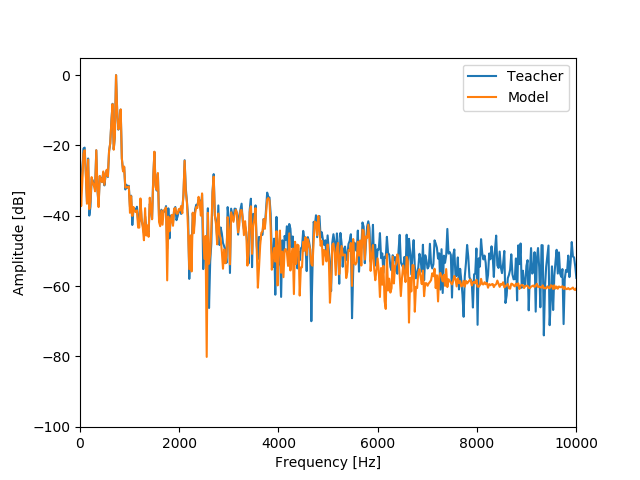
\includegraphics[width=90mm]{gain5_fft_hikaku2.png}
 \end{center}
   \subcaption{音声2}
 \label{fig:two}
 \end{minipage}
 \caption{DIST:5 教師データ,モデル出力周波数スペクトル比較}
\end{figure}

\begin{figure}[htbp]
 \begin{minipage}{0.5\hsize}
 \begin{center}
  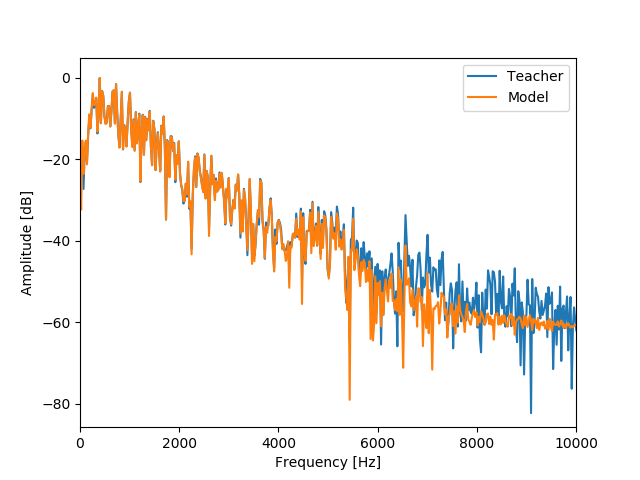
\includegraphics[width=90mm]{gain10_fft_hikaku.png}
 \end{center}
   \subcaption{音声1}
 \label{fig:one}
 \end{minipage}
 \begin{minipage}{0.5\hsize}
 \begin{center}
  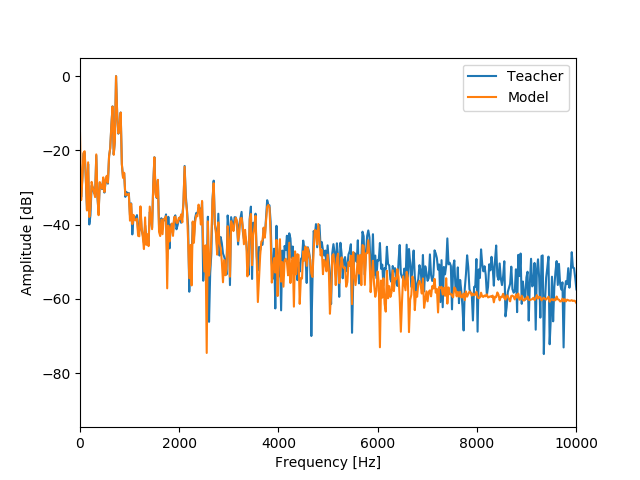
\includegraphics[width=90mm]{gain10_fft_hikaku2.png}
 \end{center}
   \subcaption{音声1}
 \label{fig:two}
 \end{minipage}
 \caption{DIST:9 教師データ,モデル出力周波数スペクトル比較}
\end{figure}

\begin{figure}[htbp]
 \begin{minipage}{0.5\hsize}
 \begin{center}
  \includegraphics[width=90mm]{tone1_fft.png}
 \end{center}
   \subcaption{音声1}
 \label{fig:one}
 \end{minipage}
 \begin{minipage}{0.5\hsize}
 \begin{center}
  \includegraphics[width=90mm]{tone1_fft2.png}
 \end{center}
   \subcaption{音声1}
 \label{fig:two}
 \end{minipage}
 \caption{TONE:1 教師データ,モデル出力周波数スペクトル比較}
\end{figure}

\begin{figure}[htbp]
 \begin{minipage}{0.5\hsize}
 \begin{center}
  \includegraphics[width=90mm]{tone10_fft.png}
 \end{center}
   \subcaption{音声1}
 \label{fig:one}
 \end{minipage}
 \begin{minipage}{0.5\hsize}
 \begin{center}
  \includegraphics[width=90mm]{tone10_fft2.png}
 \end{center}
   \subcaption{音声1}
 \label{fig:two}
 \end{minipage}
 \caption{TONE:9 教師データ,モデル出力周波数スペクトル比較}
\end{figure}

\newpage
\section{推論にかかる時間の測定}
5秒間の音源をモデルに入力し,推論された出力が保存されるまでの時間を5回測定し,平均を算出した.測定結果を表5.6 に示す.入力音源の時間長の3倍以上の時間がかかっていることがわかる.

\begin{table}[htbp]
  \begin{center}
  \caption{推論にかかる時間測定結果}
  \begin{tabular}{c|c} \hline
    回数&測定時間[s]\\ \hline
    1&17.785 \\
    2&17.956 \\
    3&17.683 \\
    4&17.580 \\
    5&17.854 \\ \hline
    平均&17.772\\ \hline
  \end{tabular}
  \end{center}
\end{table}

\chapter{考察}
本研究では,ニューラルネットワークを用いることでPC のみで動作し,シミュレートする対象となるエフェクタの入出力音を入れるだけで,音響フィルタを手軽にシミュレートできるシミュレータ開発の検討を行った.

DS-1のDISTのつまみを変えた3パターンの教師データを学習させた結果,図5.1~5.5より,どのパターンも損失が収束したことがわかる.
損失の値が小さいほど回帰モデルが出力する値は真に近くなり,高い精度の実現を示す.epochsを重ねるごとに教師データ,テストデータ共に損失は減少しているため,学習に成功していることを示す.

次に,エフェクタ実機から出力された音声と,学習させたニューラルネットワークから出力された音声波形の概形の比較を行った.
DS-1の出力波形と学習済みモデルの出力波形を比較すると,図5.6~5.10より,どのパターンのモデルも,概ね教師信号に追従した波形を出力していることがわかる.
DIST:5,DIST:9はDIST:1,TONE:1,TONE:9よりも教師データとモデルの出力の波形のずれが大きくなる傾向にある.

しかし,これらの出力信号にフーリエ変換処理を行った後に比較すると,図5.11~5.15より,どのパターンも6000 Hz以降の再現度が著しく低下していることがわかる.
原因としては,教師データ不足やサンプリング周波数の低さなどが考えられる.学習データが少ない場合,情報が比較的スパースである高域の修復性能が劣化するという問題が発生する.高域の精度低下の問題については,ギター以外の信号を使うことによる多様な教師データの追加や,モデルのハイパーパラメータの最適化などを行うことで解決が期待できる.

リアルタイムでの動作を視野に入れ,推論にかかる時間を測定した.表5.6 より,現環境では,推論には入力音源の時間長の3倍以上の時間がかかることがわかる.
リアルタイムで入力された音声を変換し出力するシステムの構築には,サンプリング周波数の削減や,強力なプロセッサの使用などで推論の速度を上げる必要がある.
入力音源の時間長の等倍以下の時間で推論する速度が必要である.

本研究で,PCのみで動作するシミュレータを構築し,エフェクタへの入出力音を用意しソフトウェアで学習させることで,ある程度の精度が得られることを実証した.
今後の課題としては,人間の耳で聴取実験を行い,より細かくシミュレータを評価する必要がある.また,ギター演奏の未経験者と経験者では,実験結果に差異が表れるかを明らかにする必要もある.

\begin{thebibliography}{3}
  \bibitem{sinco} 株式会社シンコーミュージック・エンタテインメント: "THE OVERDRIVE BOOK2 増補・改訂版",pp.19-28 (2008).
  \bibitem{torpido} 日本エレクトロ・ハーモニックス株式会社ホームページ,http://www.electroharmonix.co.jp/twonotes/index.html
  \bibitem{ninsiki} Chung-Cheng Chiu, Tara N. Sainath, Yonghui Wu, Rohit Prabhavalkar, Patrick Nguyen, Zhifeng Chen, Anjuli Kannan, Ron J. Weiss, Kanishka Rao, Katya Gonina, Navdeep Jaitly, Bo Li, Jan Chorowski, Michiel Bacchiani: "STATE-OF-THE-ART SPEECH RECOGNITION WITH SEQUENCE-TO-SEQUENCE MODELS" (2017).
  \bibitem{gousei} Aaron van den Oord, Yazhe Li, Igor Babuschkin, Karen Simonyan, Oriol Vinyals, Koray Kavukcuoglu: "Parallel WaveNet:Fast High-Fidelity Speech Synthesis" (2017).
  \bibitem{RNN} 巣籠悠輔: "詳解ディープラーニング",マイナビ出版, pp.209-250 (2017).
\end{thebibliography}

\end{document}
